\documentclass[border=4pt,crop=true]{standalone}
\usepackage{pgfplots}
\pgfplotsset{compat=1.18}

\begin{document}
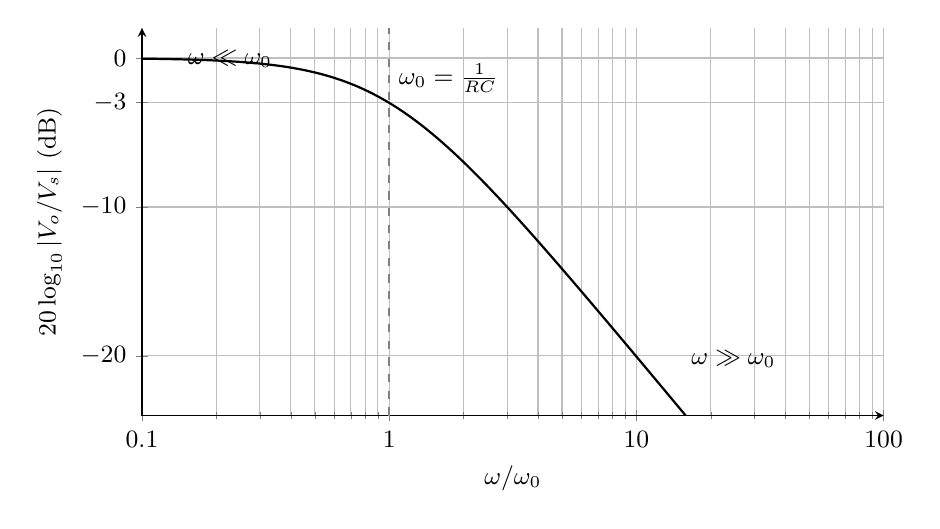
\begin{tikzpicture}
  \begin{axis}[
    width=11cm,
    height=6.5cm,
    xmode=log,
    xmin=1e-1,
    xmax=1e2,
    ymin=-24,
    ymax=2,
    axis lines=left,
    xlabel={$\omega/\omega_0$},
    ylabel={$20\log_{10}|V_o/V_s|$ (dB)},
    xtick={1e-1,1,1e1,1e2},
    xticklabels={$0.1$,$1$,$10$,$100$},
    ytick={-20,-10,-3,0},
    grid=both,
    minor tick num=1,
    tick label style={font=\small},
    label style={font=\small},
    every axis plot/.append style={thick},
  ]
    \addplot[domain=1e-1:1e2,samples=300] {-10*ln(1+x^2)/ln(10)};
    \addplot[gray,dashed] coordinates {(1,-24) (1,2)};
    \node[anchor=south west,font=\small] at (axis cs:1,-3) {$\omega_0=\frac{1}{RC}$};
    \node[anchor=south west,font=\small] at (axis cs:0.14,-1.3) {$\omega\ll\omega_0$};
    \node[anchor=north east,font=\small] at (axis cs:40,-19) {$\omega\gg\omega_0$};
  \end{axis}
\end{tikzpicture}
\end{document}
